\documentclass{beamer}
\usepackage[utf8]{inputenc}
\usepackage[T1]{fontenc}
\usepackage{graphicx}
\usepackage{float}
\usepackage{hyperref}
\usepackage{listings}

\setbeamertemplate{navigation symbols}{}

\usetheme{Madrid}
\title{Graphs and Discrete Structures Project : The Ghost Hunter}
\author{BERGER Simon \and GROUSSON Dylan \and ERGIN Seckin-Yağmur \and ROLAND--ROUDIL Tom}
\date{7th January 2026}

\definecolor{codegreen}{rgb}{0,0.6,0}
\definecolor{codegray}{rgb}{0.5,0.5,0.5}
\definecolor{codepurple}{rgb}{0.58,0,0.82}
\definecolor{backcolour}{rgb}{0.95,0.95,0.92}

\lstdefinestyle{mystyle}{
    backgroundcolor=\color{backcolour},
    commentstyle=\color{codegreen},
    keywordstyle=\color{magenta},
    numberstyle=\tiny\color{codegray},
    stringstyle=\color{codepurple},
    basicstyle=\ttfamily\scriptsize,
    breakatwhitespace=false,
    breaklines=true,
    captionpos=b,
    keepspaces=true,
    numbers=left,
    numbersep=5pt,
    showspaces=false,
    showstringspaces=false,
    showtabs=false,
    tabsize=2
}

\lstset{style=mystyle}

\begin{document}

\begin{frame}
\titlepage
\end{frame}

\begin{frame}
\frametitle{Overview}
\begin{itemize}
    \item A Java-based simulator for the ``Ghost Hunter'' game on graphs.
    \item \textbf{Goal}: Empirically test and validate conjectures about hunter strategies.
    \item Provides statistical results on the effectiveness of different policies.
    \item \textbf{Output}: Average number of rounds to find the ghost.
\end{itemize}
\end{frame}

\begin{frame}
\frametitle{Configuration}
\begin{itemize}
    \item All parameters are set in the \texttt{config.toml} file.
    \item Key parameters:
    \begin{itemize}
        \item \texttt{nbSimu}: Number of simulations to run.
        \item \texttt{policy}: The hunter's strategy.
        \item \texttt{execType}: The execution mode (e.g., single graph, up to size N).
        \item \texttt{graphType}: The type of graph for the simulation.
    \end{itemize}
\end{itemize}
\end{frame}

\begin{frame}
\frametitle{Hunter Policies}
Three main strategies for the hunter:
\begin{itemize}
    \item \texttt{RANDOM}: Chooses a random vertex (not the previous one).
    \item \texttt{HIGH\_DEGREE\_PRIO}: Random choice with a bias towards vertices with more connections.
    \item \texttt{NEXT\_VERTEX}: Deterministic policy for cycle graphs, moving to the next vertex in sequence.
\end{itemize}
\end{frame}

\begin{frame}
\frametitle{Graph Types}
\begin{columns}[T]
    \begin{column}{.3\textwidth}
        \textbf{Graph Types}:
        \begin{itemize}
            \item \texttt{N\_CYCLE}
            \item \texttt{N\_COMP}
            \item \texttt{N\_K\_REGULAR}
            \item \texttt{N\_CONN}
            \item \texttt{FROM\_FILE}
        \end{itemize}
    \end{column}
    \begin{column}{.35\textwidth}
        \vspace{-1em}
        \begin{figure}
            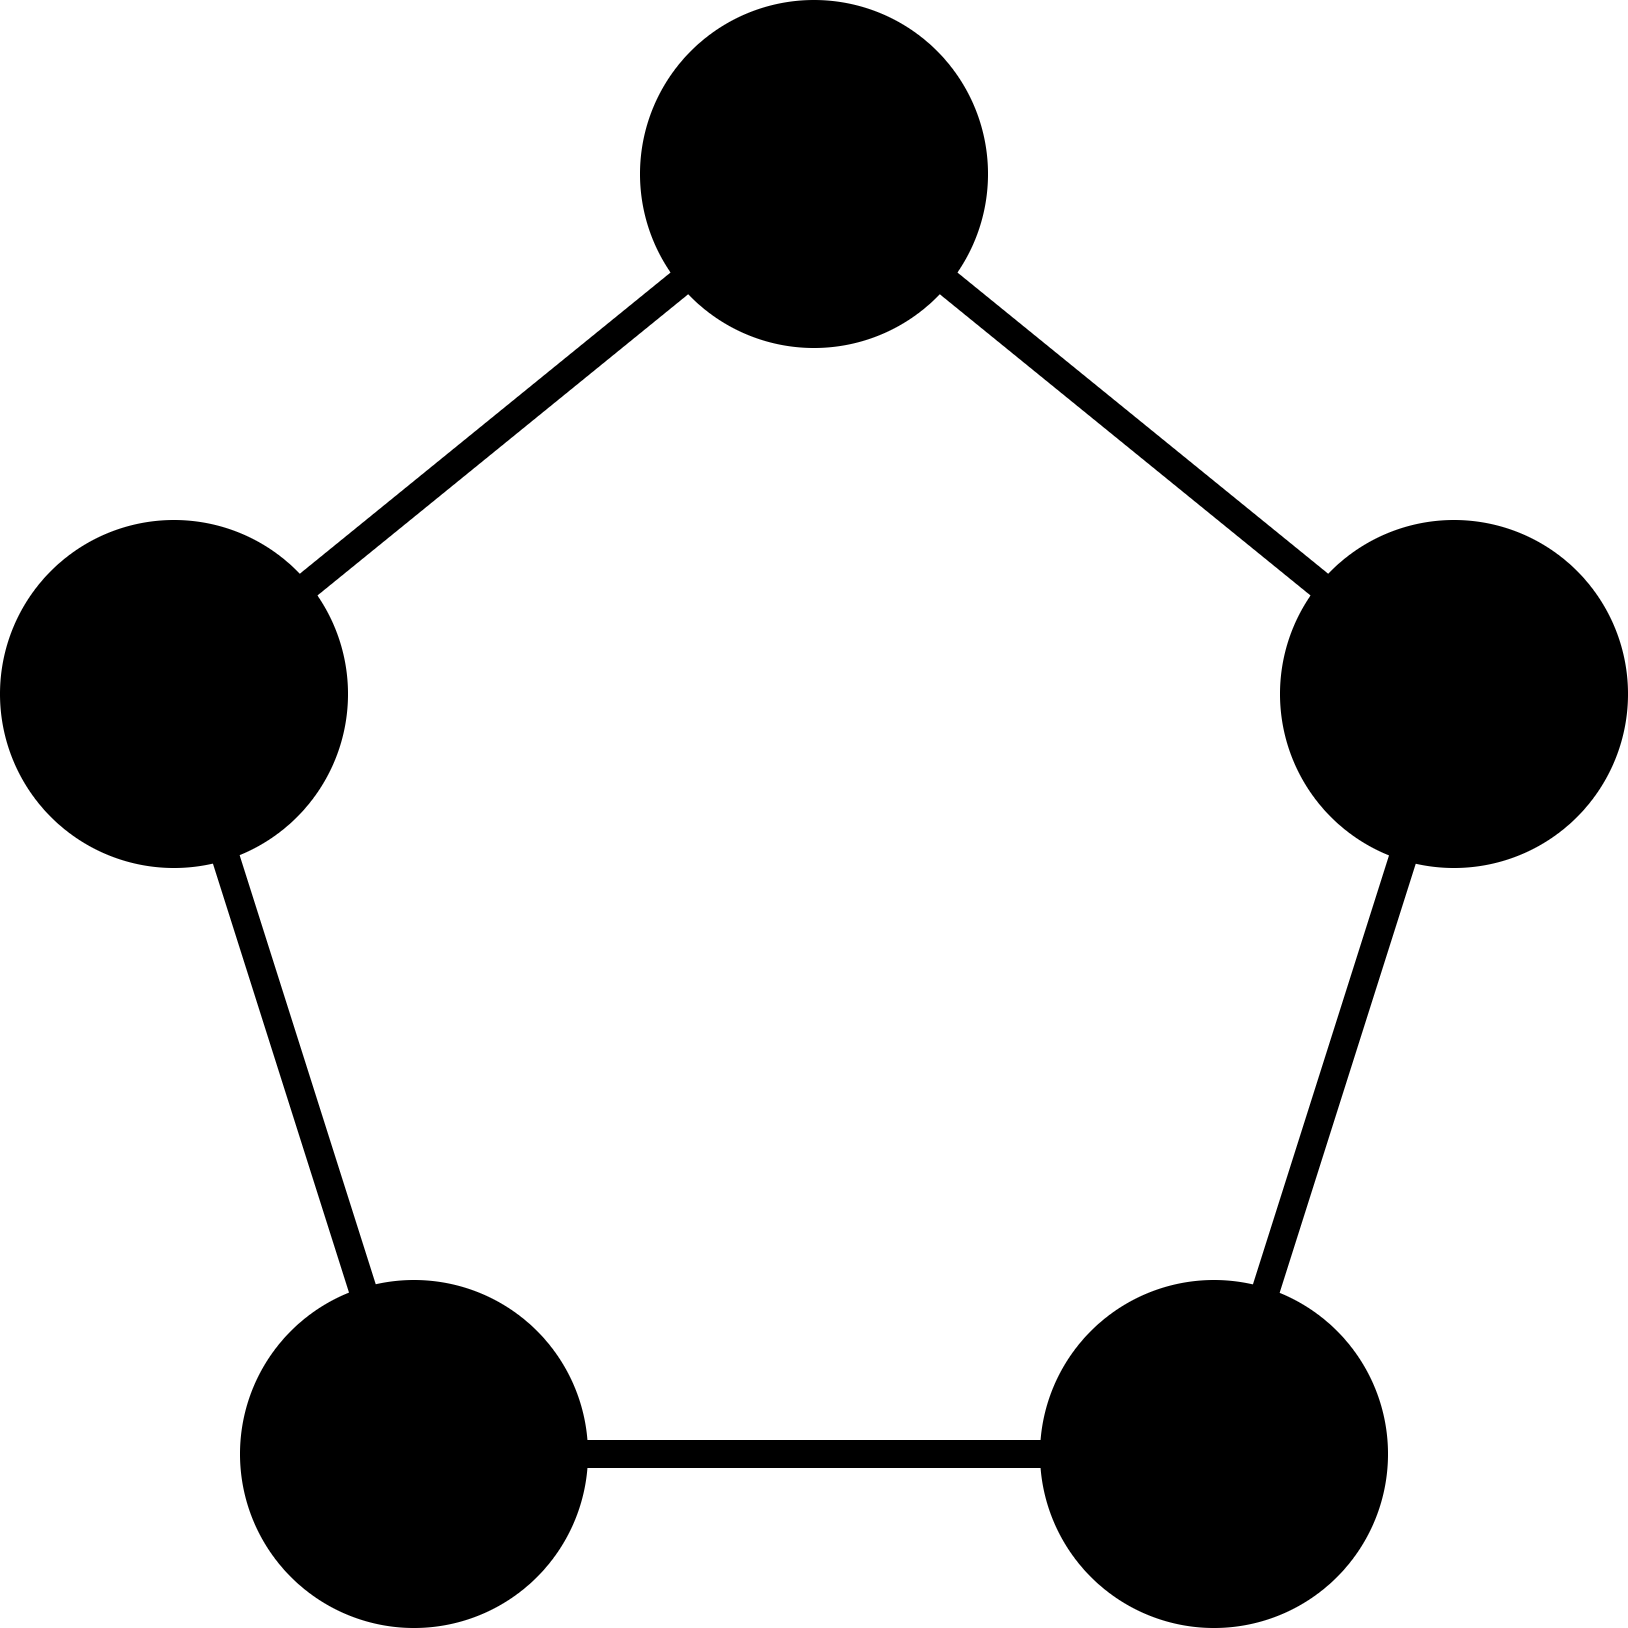
\includegraphics[width=0.6\linewidth]{images/black_5_cycle.png}
            \caption{\texttt{N\_CYCLE}}
        \end{figure}
        \vspace{-1em}
        \begin{figure}
            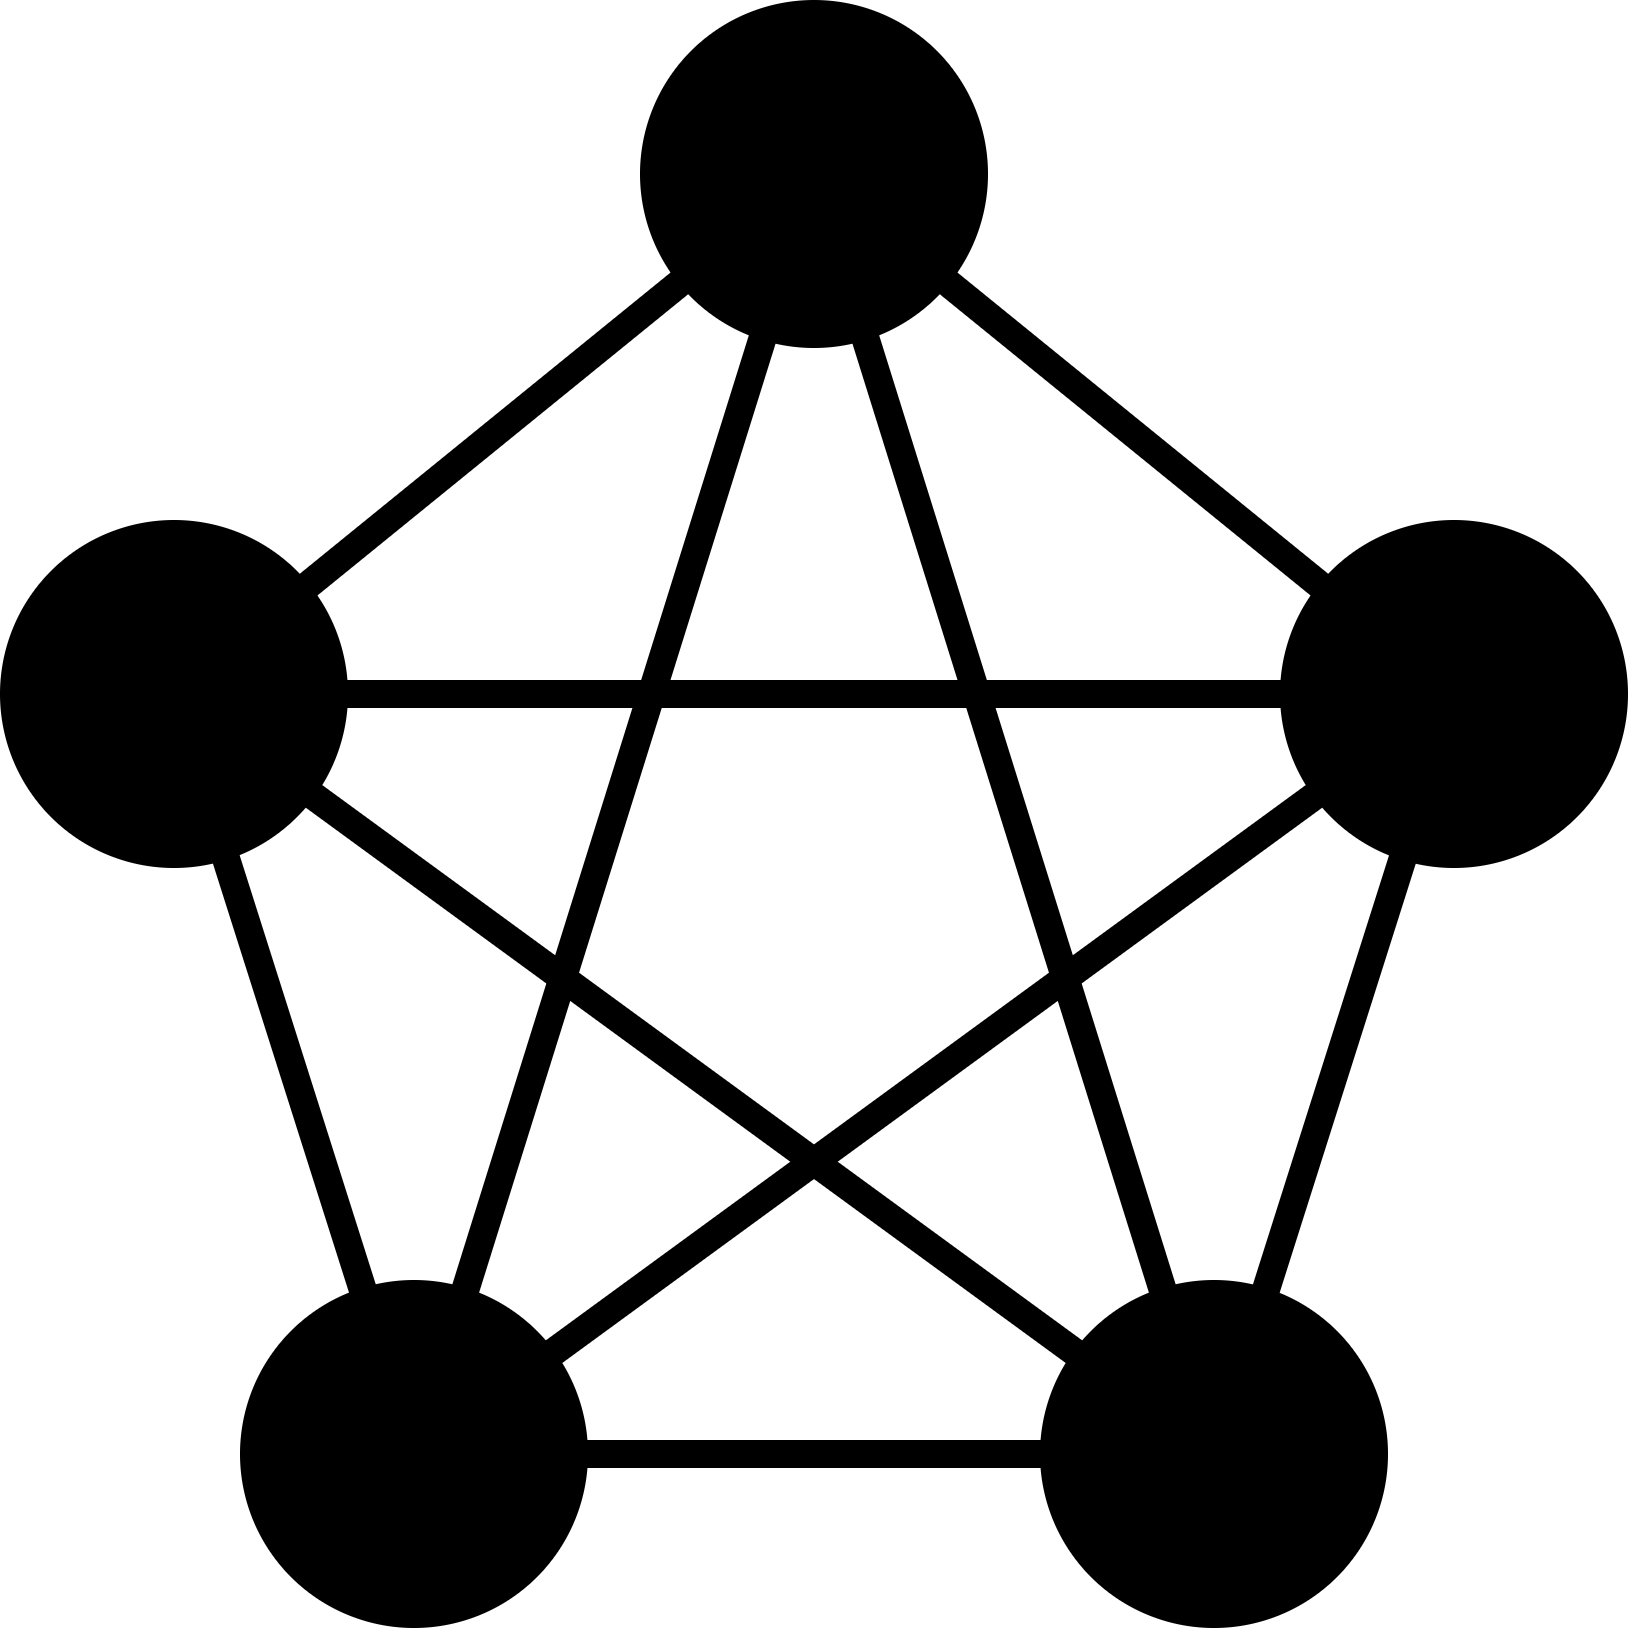
\includegraphics[width=0.6\linewidth]{images/black_5_comp.png}
            \caption{\texttt{N\_COMP}}
        \end{figure}
    \end{column}
    \begin{column}{.35\textwidth}
        \vspace{-1em}
        \begin{figure}
            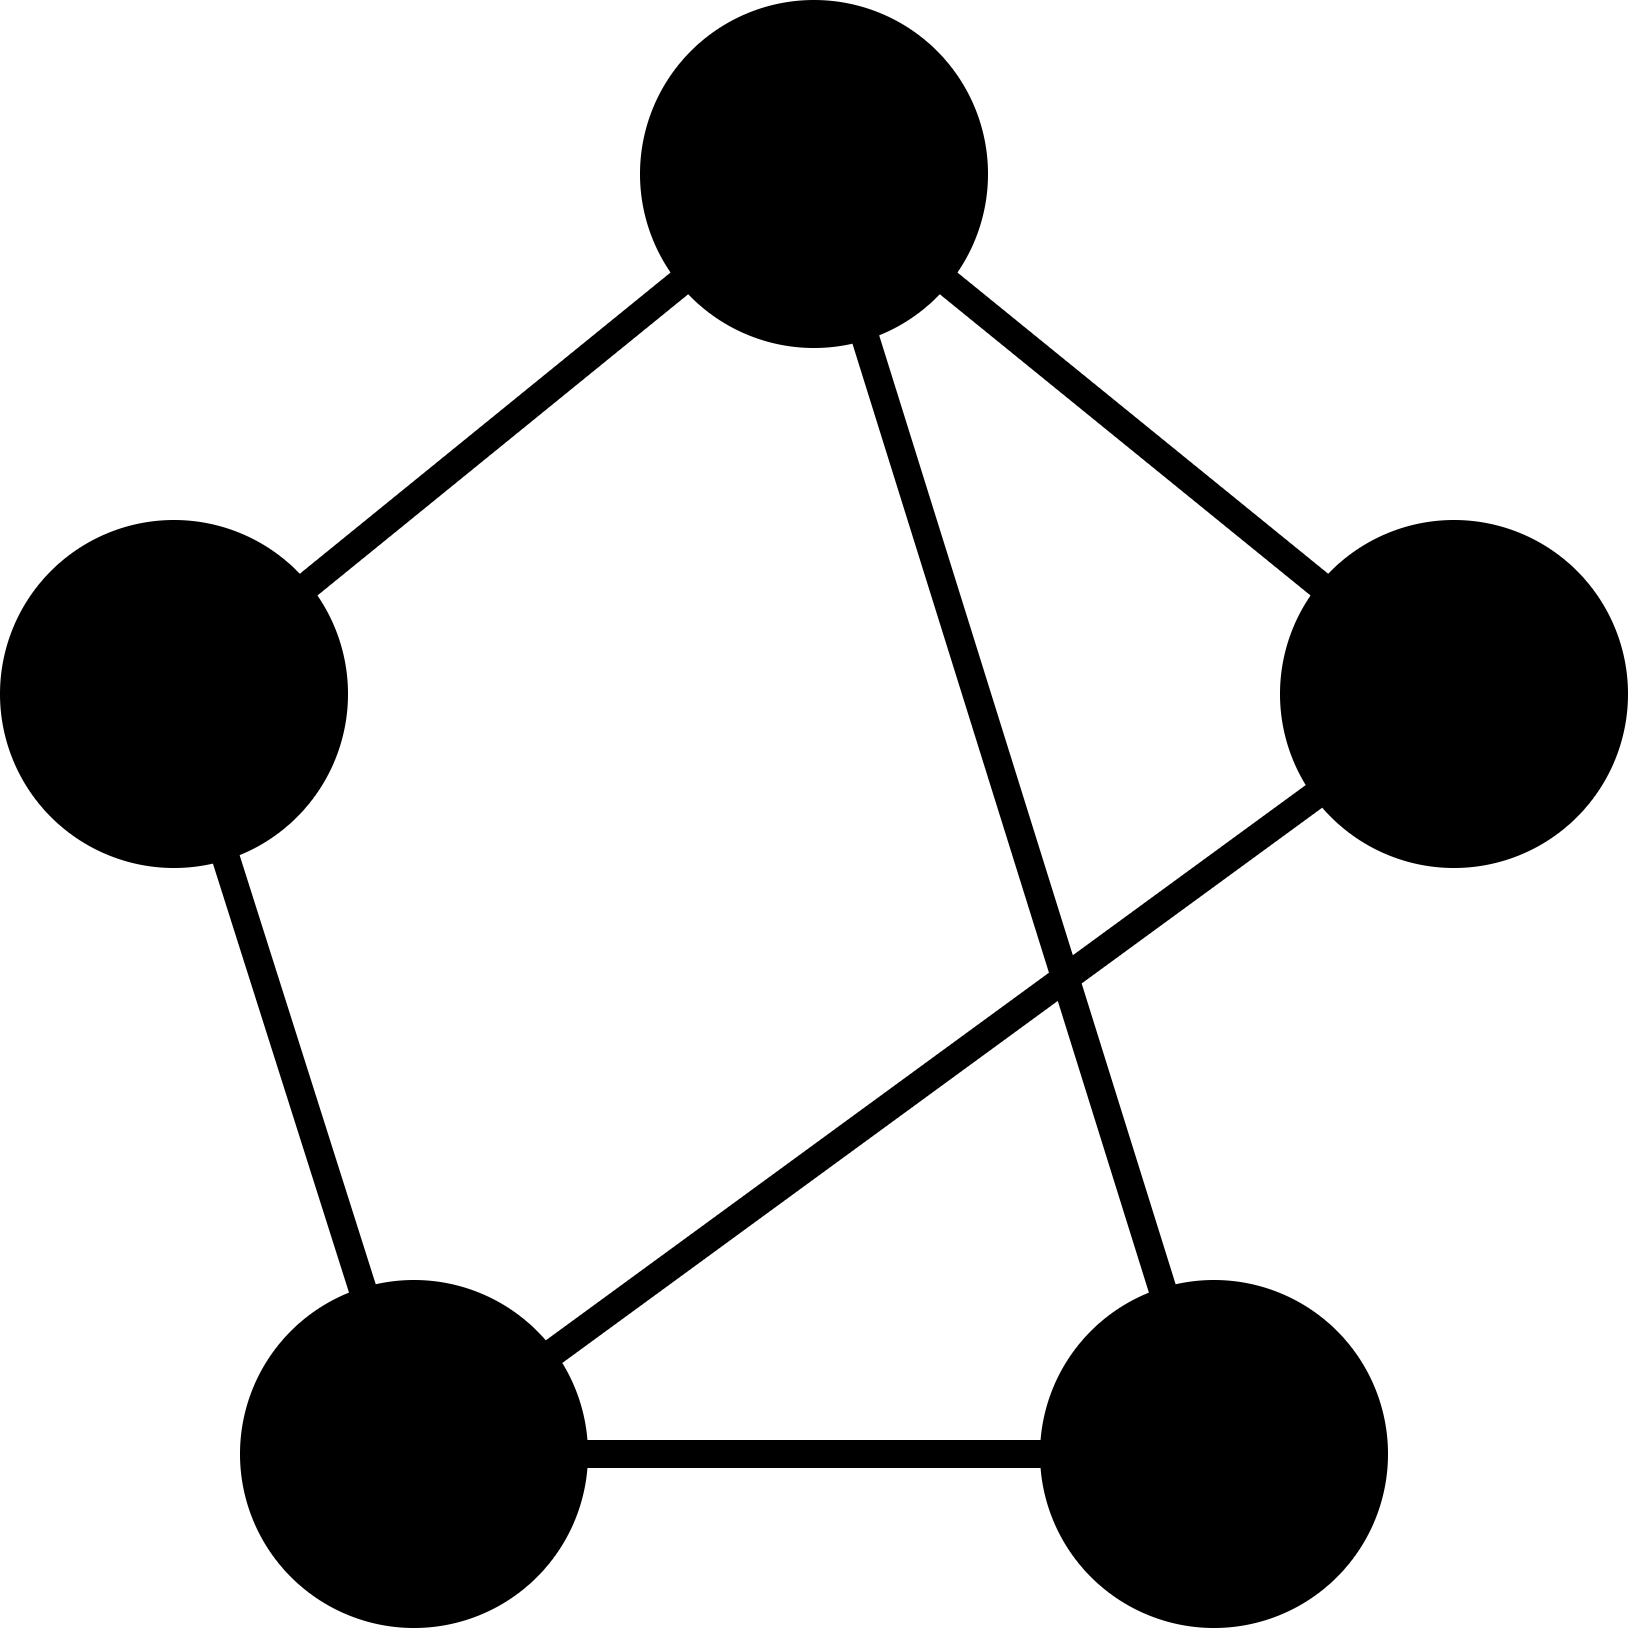
\includegraphics[width=0.6\linewidth]{images/black_5_conn.png}
            \caption{\texttt{N\_CONN}}
        \end{figure}
        \vspace{-1em}
        \begin{figure}
            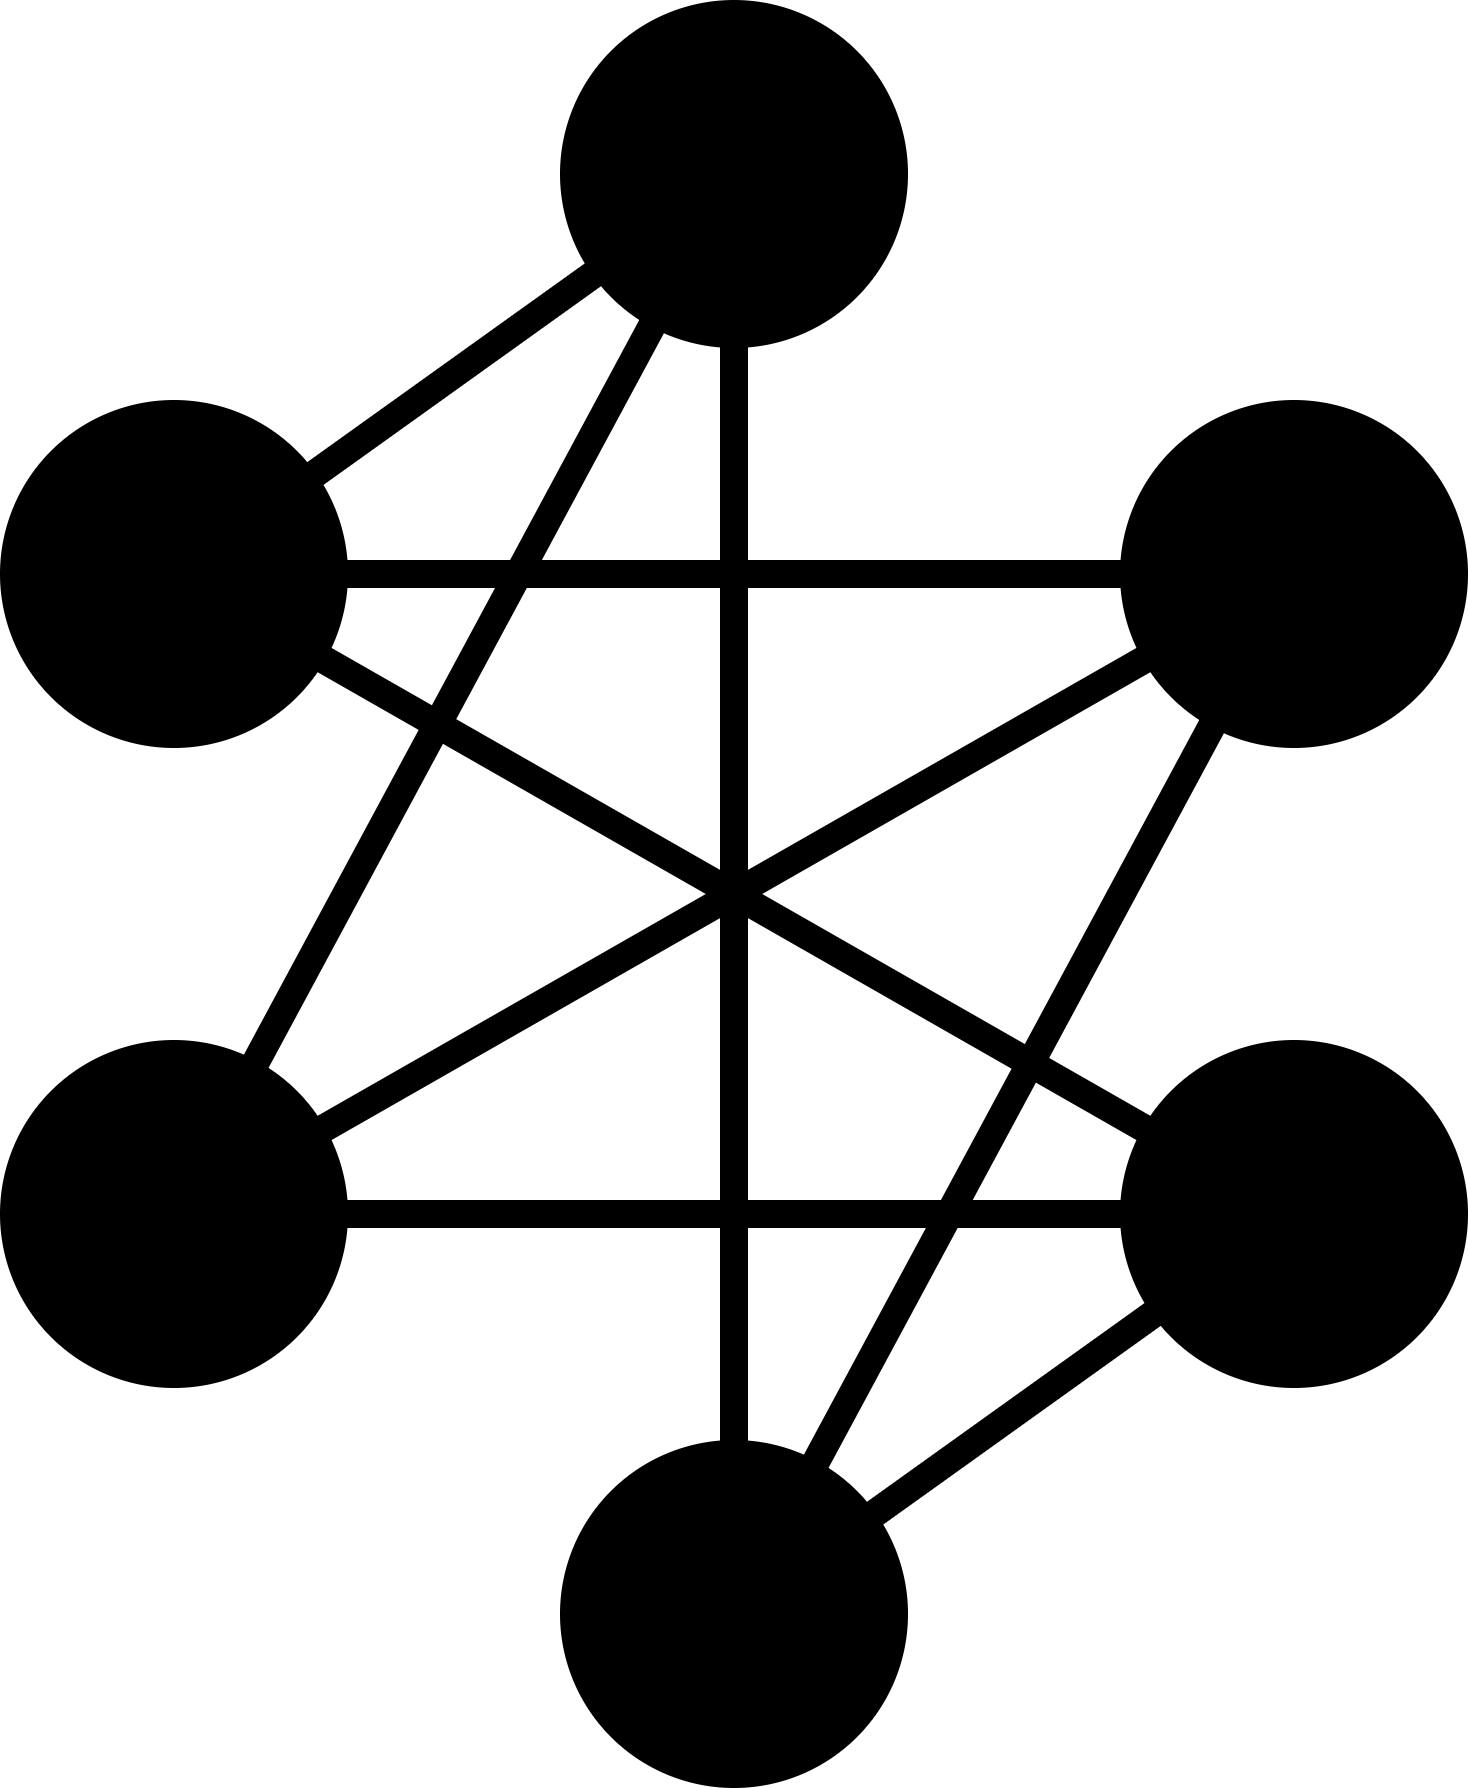
\includegraphics[width=0.6\linewidth]{images/black_6_3_regular.png}
            \caption{\texttt{N\_K\_REGULAR}}
        \end{figure}
    \end{column}
\end{columns}
\end{frame}

\end{document}
